\documentclass[tikz,10pt]{standalone}
\usepackage{amsmath,amssymb,cmap,pgfplots,pgfplotstable}
\usetikzlibrary{arrows,calc,intersections}
\pgfplotsset{compat=newest}

\begin{document} 
	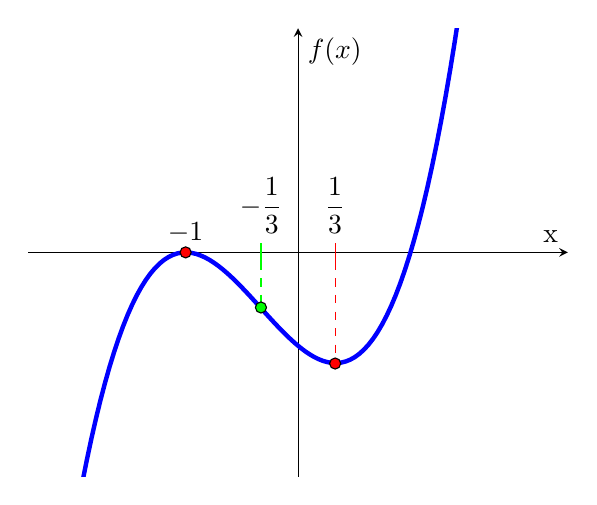
\begin{tikzpicture}
		\begin{axis}[xlabel=x, ylabel={$f(x)$}, axis lines=middle, ymax = 2, ymin = -2, xmax = 2,	xmin = -2, enlargelimits=true,xtick=\empty,	ytick=\empty]
			\addplot[blue!, line width=1.6pt,	domain={-2:2}, samples=100]{x^3 + x^2 - x -1};
			\draw[red!] (0.33,-0.1) -- (0.33,0.1) node[black!, above] {$\dfrac{1}{3}$};
			\draw[red!, dashed] (0.33,-0.1) -- (0.33,-1.19);
			\draw[fill=red] (0.33,-1.19) circle (2pt);
			\draw[fill=red] (-1,0) circle (2pt);
			\draw (-1,0) node[black, above] {$-1$};
			\draw[green!] (-0.33,-0.1) -- (-0.33,0.1) node[black!, above] {$-\dfrac{1}{3}$};
			\draw[green!, dashed] (-0.33,-0.1) -- (-0.33,-0.59);
			\draw[fill=green] (-0.33,-0.59) circle (2pt);
		\end{axis}
	\end{tikzpicture}
\end{document}